\section{熵条件}
\label{sec:cons-entropy}

弱解到底多到什么程度？怎样从中挑出合理的那一个？本节先把多余的解摆出来，再从特征线的方向和小黏性的极限两个角度找到选择规则，最后把规则写成对一切弱解都能检验的不等式。

\paragraph{同一初值的无穷多个弱解}
仍取Burgers方程和阶跃初值$u_0=0$（$x<0$）、$u_0=1$（$x>0$）。上一节的两个解只是一族解的两端。任取$\alpha\in[0,1]$，令
\begin{equation}
  u^{\alpha}(x,t)=\begin{cases}
    0,&x<\alpha t/2,\\
    \alpha,&\alpha t/2<x<\alpha t,\\
    x/t,&\alpha t<x<t,\\
    1,&x\geq t.
  \end{cases}
  \label{eq:cons-weak-family}
\end{equation}

逐块检验。常数块上两个偏导都是零，方程成立；块$u=x/t$上
\[
  \partial_tu+u\,\partial_xu=-\frac{x}{t^2}+\frac{x}{t}\cdot\frac1t=0 .
\]
唯一的跳跃在$x=\alpha t/2$处，两侧是$0$和$\alpha$，由式~\eqref{eq:cons-burgers-speed}，速度应为$\alpha/2$，正好相符。其余两条接缝连续。由定理~\ref{thm:cons-rh}，每个$u^{\alpha}$都是弱解。

图~\ref{fig:cons-weak-family}画出$\alpha=1,\,1/2,\,0$三种情形。$\alpha=1$就是$u^{\mathrm{j}}$，$\alpha=0$就是$u^{\mathrm{f}}$，中间的$\alpha$把一部分扇形换成了向上的跳跃。

\begin{BookInlineFigure}
  \centering
  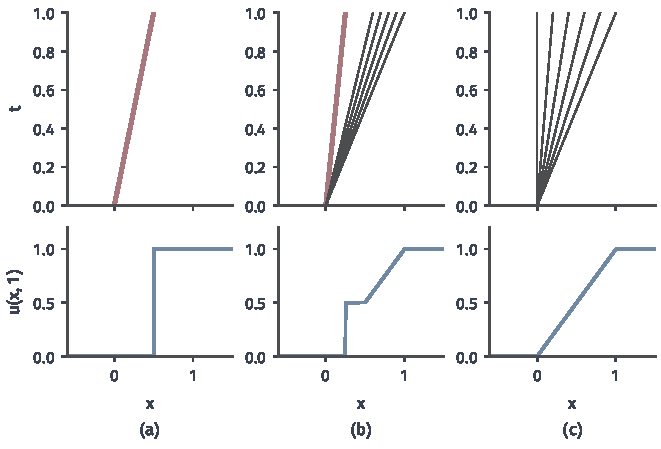
\includegraphics[width=112mm]{figures/06-differential-equations/02-partial-differential-equations/matplotlib/cons-weak-family/figure.pdf}
  \caption{阶跃初值的弱解族~\eqref{eq:cons-weak-family}。上排是$(x,t)$平面，红色粗线是向上的跳跃，细线是扇形中的特征线；下排是$t=1$的形状。(a)$\alpha=1$，全部是跳跃。(b)$\alpha=1/2$，跳跃接扇形。(c)$\alpha=0$，全部是扇形，没有跳跃。}
  \label{fig:cons-weak-family}
\end{BookInlineFigure}

更极端的例子是零初值。任取$b>0$，令
\begin{equation}
  u(x,t)=\begin{cases}
    0,&x<-bt/2,\\
    -b,&-bt/2<x<0,\\
    b,&0<x<bt/2,\\
    0,&x>bt/2.
  \end{cases}
  \label{eq:cons-zero-data}
\end{equation}

三条跳跃线的速度都满足式~\eqref{eq:cons-burgers-speed}：$0$与$-b$之间是$-b/2$，$-b$与$b$之间是$0$，$b$与$0$之间是$b/2$。$t=0$时$u$处处为零，所以这是零初值的非零弱解，见图~\ref{fig:cons-zero-data}。静止的流体从原点自发地向两边散开，总量却分毫不差。所以只算收支账排除不了这样的解。

\begin{BookInlineFigure}
  \centering
  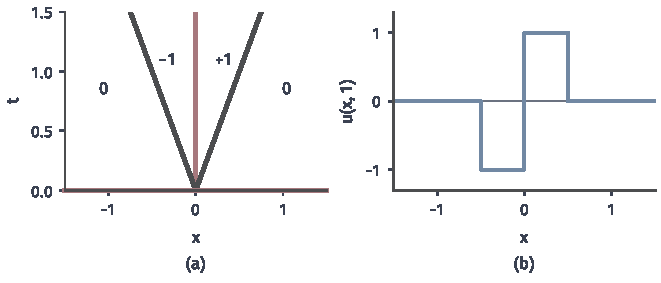
\includegraphics[width=112mm]{figures/06-differential-equations/02-partial-differential-equations/matplotlib/cons-zero-data/figure.pdf}
  \caption{零初值的非零弱解，$b=1$。(a)$(x,t)$平面，数字是各区域的值，红色粗线$x=0$是向上的跳跃，两条深灰粗线是向下的跳跃。(b)$t=1$的形状，正负两块面积相互抵消。}
  \label{fig:cons-zero-data}
\end{BookInlineFigure}

\paragraph{特征线必须汇入间断}
看特征线在间断两侧的走向就能分出好坏。先看图~\ref{fig:cons-lax-in-out}(a)，其中$u_-=1$、$u_+=0$，$s=1/2$。左侧特征线的速度$1$大于$s$，从后面追上间断；右侧特征线的速度$0$小于$s$，被间断追上。两侧的特征线都汇入间断，间断两侧的状态都由更早的初值决定。

(b)中$u_-=0$、$u_+=1$，$s$同样是$1/2$，方向却反了：左侧速度$0$小于$s$，右侧速度$1$大于$s$，特征线都从间断上离开。这些特征线沿途携带的值并不来自初值，只能在间断线上凭空产生。这就是前面的解不唯一的根源：既然这些值无从确定，它们就可以任意选取。

\begin{BookInlineFigure}
  \centering
  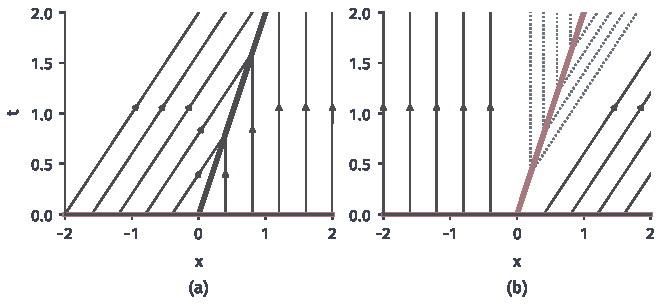
\includegraphics[width=112mm]{figures/06-differential-equations/02-partial-differential-equations/matplotlib/cons-lax-in-out/figure.pdf}
  \caption{两种间断两侧的特征线，$s$都是$1/2$，箭头指向时间增大的方向。(a)$u_-=1$、$u_+=0$（深灰粗线），两侧特征线都汇入。(b)$u_-=0$、$u_+=1$（红色粗线），点线表示从间断上发出的特征线，初值决定不了它们的取值。}
  \label{fig:cons-lax-in-out}
\end{BookInlineFigure}

把这一观察写成条件，就是\term{Lax熵条件}（Lax entropy condition）：
\begin{equation}
  F'(u_-)>s>F'(u_+).
  \label{eq:cons-lax}
\end{equation}

满足这一条件的间断称为\term{激波}（shock wave）。$F$严格凸时条件有更简单的形式。此时$F'$严格递增，$s$是$F'$在$u_-$与$u_+$之间的平均，严格落在两端值之间。所以当$u_-\neq u_+$时，式~\eqref{eq:cons-lax}等价于$F'(u_-)>F'(u_+)$，也就是$u_->u_+$。

对Burgers方程这句话是说，只有向下的跳跃才允许存在。检验前面的例子：$(u_-,u_+)=(1,0)$满足$1>1/2>0$；$(0,1)$要求$0>1/2>1$，不成立。凹的车流通量则相反，要求$u_-<u_+$：前方密度大、后方密度小，正是车辆追上堵车队尾的情形。例如$u_-=0.2$、$u_+=0.8$时
\[
  s=\frac{0.16-0.16}{0.6}=0,\qquad F'(0.2)=0.6>0>-0.6=F'(0.8),
\]
队尾静止不动，两侧的扰动都汇向队尾。

式~\eqref{eq:cons-lax}只适用于分段光滑的解和凸通量。要对一般的有界解下定义，得从这条规则的来源说起。

\paragraph{消失黏性}
真实的流体和车流都有一点扩散：司机会根据前方密度提前调整。在方程里加上小的黏性项，
\begin{equation}
  \partial_tu^{\nu}+\partial_xF(u^{\nu})=\nu\,\partial_{xx}u^{\nu},\qquad \nu>0.
  \label{eq:cons-viscous}
\end{equation}
式~\eqref{eq:cons-viscous}是抛物型方程，第~\ref{chap:diffusion-equations}章的抹平作用使它的解保持光滑，也没有多解的问题。合理的弱解应该是$\nu\to0$时的极限。这种通过\term{消失黏性}（vanishing viscosity）挑选解的做法，可以在Burgers方程上算到底。

寻找行波解$u^{\nu}=U(\xi)$，$\xi=x-st$，$U(\pm\infty)=u_\pm$。代入Burgers方程，得到
\[
  -sU'+UU'=\nu U'' .
\]

对$\xi$积分一次，积分常数记为$C$：
\[
  -sU+\frac{U^2}{2}=\nu U'+C .
\]

令$\xi\to\pm\infty$，$U'\to0$，两端各给一个等式：
\[
  C=-su_-+\frac{u_-^2}{2}=-su_++\frac{u_+^2}{2}.
\]
当$u_-\neq u_+$时，消去$C$得到$s=(u_-+u_+)/2$，Rankine--Hugoniot条件自动出现。把$s$与$C=-u_-u_+/2$代回，一阶方程化为
\begin{equation}
  \nu U'=\frac12(U-u_-)(U-u_+).
  \label{eq:cons-viscous-profile}
\end{equation}

右端在$U$介于$u_-$与$u_+$之间时为负，所以$U$只能沿$\xi$递减。从$\xi=-\infty$的$u_-$走到$\xi=+\infty$的$u_+$，就必须$u_->u_+$。向上的跳跃没有黏性剖面，向下的跳跃才有。解出这个分离变量方程，得到
\begin{equation}
  U(\xi)=\frac{u_-+u_+}{2}-\frac{u_--u_+}{2}\tanh\frac{(u_--u_+)\,\xi}{4\nu}.
  \label{eq:cons-viscous-tanh}
\end{equation}

过渡层的宽度约为$4\nu/(u_--u_+)$，$\nu\to0$时剖面收缩成跳跃，见图~\ref{fig:cons-viscous-profile}。这是黏性对向下跳跃的解释：很薄的一层里，压缩和扩散互相平衡。

\begin{BookInlineFigure}
  \centering
  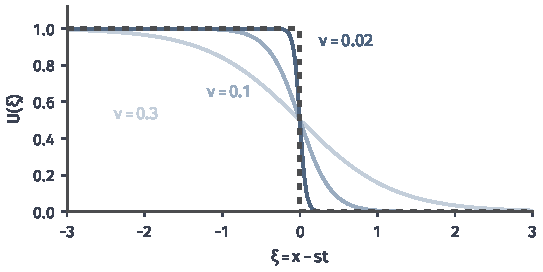
\includegraphics[width=92mm]{figures/06-differential-equations/02-partial-differential-equations/matplotlib/cons-viscous-profile/figure.pdf}
  \caption{Burgers方程的黏性行波~\eqref{eq:cons-viscous-tanh}，$u_-=1$、$u_+=0$。蓝色由浅到深是$\nu=0.3,0.1,0.02$，深灰点线是$\nu\to0$的极限跳跃。}
  \label{fig:cons-viscous-profile}
\end{BookInlineFigure}

向上的阶跃又如何？图~\ref{fig:cons-viscous-fan}把式~\eqref{eq:cons-viscous}从阶跃初值$0$、$1$开始算到$t=1$。数值解没有靠近跳跃$u^{\mathrm{j}}$，而是贴向连续的扇形$u^{\mathrm{f}}$。在弱解族~\eqref{eq:cons-weak-family}中，黏性选中的是$\alpha=0$。

\begin{BookInlineFigure}
  \centering
  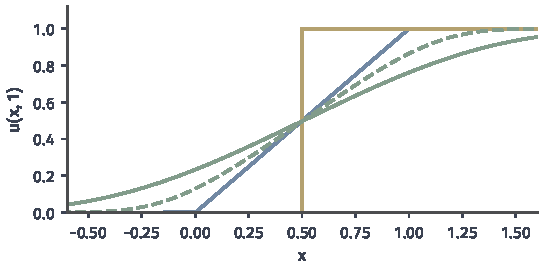
\includegraphics[width=92mm]{figures/06-differential-equations/02-partial-differential-equations/matplotlib/cons-viscous-fan/figure.pdf}
  \caption{阶跃初值$0$、$1$的黏性解在$t=1$的形状，由守恒的显式差分格式算出。绿色实线和虚线是$\nu=0.1$和$\nu=0.02$，蓝线是扇形解$u^{\mathrm{f}}$，黄线是跳跃解$u^{\mathrm{j}}$。$\nu$减小时数值解靠向蓝线。}
  \label{fig:cons-viscous-fan}
\end{BookInlineFigure}

\paragraph{熵不等式}
小黏性留下了什么可以在极限中保存的信息？取任意$C^2$凸函数$\eta$，再取$q$使$q'=\eta'F'$。这样的一对$(\eta,q)$称为\term{熵对}（entropy pair），$\eta$是熵，$q$是\term{熵通量}（entropy flux）。方程~\eqref{eq:cons-viscous}乘以$\eta'(u^{\nu})$，用链式法则整理：
\[
  \partial_t\eta(u^{\nu})+\partial_xq(u^{\nu})
  =\nu\,\partial_{xx}\eta(u^{\nu})-\nu\,\eta''(u^{\nu})\,(\partial_xu^{\nu})^2 .
\]

最后一项因为$\eta$凸而非正，它记录了扩散带来的耗散，正是这一项在极限中留下了方向。乘以$\varphi\geq0$并积分，分部积分后丢掉非负的耗散项，得到
\[
  \iint\bigl(\eta(u^{\nu})\,\partial_t\varphi+q(u^{\nu})\,\partial_x\varphi\bigr)\,\mathrm{d}x\,\mathrm{d}t
  \geq-\nu\iint\eta(u^{\nu})\,\partial_{xx}\varphi\,\mathrm{d}x\,\mathrm{d}t .
\]
假定$u^{\nu}$一致有界且几乎处处收敛，令$\nu\to0$，右端趋于零，留下一个不含$\nu$的不等式。这段推导只说明了不等式的来源，下面把它取作定义。

\begin{definition}[熵解]
\label{def:cons-entropy-solution}
设$F\in C^1(\mathbb{R})$，$u_0\in L^{\infty}(\mathbb{R})$。函数$u\in L^{\infty}(\mathbb{R}\times(0,\infty))$称为问题~\eqref{eq:cons-law}、\eqref{eq:cons-initial}的\term{熵解}（entropy solution），若对每个$C^2$凸函数$\eta$、满足$q'=\eta'F'$的$q$，以及每个非负的$\varphi\in C_c^{\infty}(\mathbb{R}\times(0,\infty))$，
\begin{equation}
  \int_0^{\infty}\!\!\int_{\mathbb{R}}\bigl(\eta(u)\,\partial_t\varphi+q(u)\,\partial_x\varphi\bigr)\,\mathrm{d}x\,\mathrm{d}t\geq0 ,
  \label{eq:cons-entropy-ineq}
\end{equation}
并且对每个$R>0$，初值在下述意义下取到：
\begin{equation}
  \operatorname*{ess\,lim}_{t\downarrow0}\int_{-R}^{R}\lvert u(x,t)-u_0(x)\rvert\,\mathrm{d}x=0 .
  \label{eq:cons-entropy-initial}
\end{equation}
\end{definition}

不等式~\eqref{eq:cons-entropy-ineq}是$\partial_t\eta(u)+\partial_xq(u)\leq0$的弱形式。取$\eta(u)=u$、$q=F$和$\eta(u)=-u$、$q=-F$，两者都是凸的，两个不等式合起来给出等式，再结合式~\eqref{eq:cons-entropy-initial}，熵解一定是弱解。$C^1$解由链式法则使式~\eqref{eq:cons-entropy-ineq}取等号，所以经典解也是熵解。

“熵”的名字来自气体动力学，那里的物理熵经过激波只增不减；数学上取凸函数，符号相反，所以$\eta$的总量只减不增。凸性的作用是把扩散耗散的符号固定下来。可以把$\eta(u)$想成一种能量：光滑时它和$u$一样守恒，只在间断处被消耗。

\paragraph{跨间断的熵不等式}
分段光滑的解要满足什么条件？重复定理~\ref{thm:cons-rh}的散度计算，把$(u,F(u))$换成$(\eta(u),q(u))$。在间断线两侧光滑部分的贡献为零，只留下线积分，于是式~\eqref{eq:cons-entropy-ineq}等价于
\begin{equation}
  q(u_+)-q(u_-)-s\bigl(\eta(u_+)-\eta(u_-)\bigr)\leq0 .
  \label{eq:cons-jump-entropy}
\end{equation}

左端是单位时间内在间断上产生的熵。取Burgers方程、$\eta=u^2/2$、$q=u^3/3$，并用$s=(u_-+u_+)/2$。记$\Delta=u_+-u_-$，直接展开：
\[
  \begin{aligned}
    \frac{u_+^3-u_-^3}{3}-\frac{(u_-+u_+)(u_+^2-u_-^2)}{4}
    &=\Delta\,\frac{4(u_+^2+u_+u_-+u_-^2)-3(u_-+u_+)^2}{12}\\
    &=\frac{\Delta^3}{12}.
  \end{aligned}
\]

所以间断上的能量变化率恰好是
\begin{equation}
  \frac{(u_+-u_-)^3}{12},
  \label{eq:cons-energy-rate}
\end{equation}
它非正当且仅当$u_+\leq u_-$。向下的跳跃消耗能量，向上的跳跃产生能量。

用斜坡解~\eqref{eq:cons-ramp-shock}核对一下。$t\geq1$时，在包含间断的大区间上，$\int u^2/2\,\mathrm{d}x$的增长率是$1/4$，因为$u=1$的区域以速度$1/2$延伸，每单位长度带能量$1/2$。左端流入能量的速率是$q(1)=1/3$。两者相差
\[
  \frac13-\frac14=\frac{1}{12},
\]
正是式~\eqref{eq:cons-energy-rate}在$(u_-,u_+)=(1,0)$时给出的耗散率。

零初值的解~\eqref{eq:cons-zero-data}同样可以算账。中间的跳跃$-b\to b$产生能量$(2b)^3/12=2b^3/3$，两侧的跳跃各消耗$b^3/12$，净产生率为$b^3/2$，这正是总能量$b^3t/2$的增长率。这个解违反熵不等式，错就错在中间那条向上的跳跃。

图~\ref{fig:cons-energy-decay}显示贯穿例子的情况：$T^{*}$之前能量守恒，激波形成之后能量按式~\eqref{eq:cons-energy-rate}减少，而总量一直不变。这是守恒律与熵的区别：总量是真正守恒的量，熵只有在光滑时才守恒。

\begin{BookInlineFigure}
  \centering
  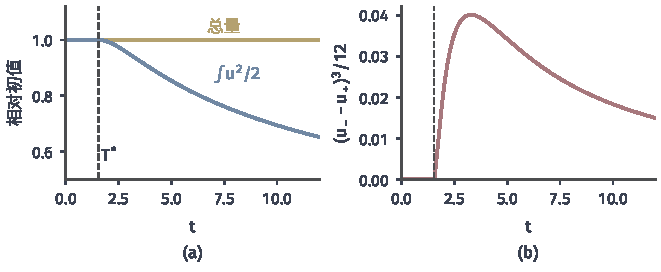
\includegraphics[width=112mm]{figures/06-differential-equations/02-partial-differential-equations/matplotlib/cons-energy-decay/figure.pdf}
  \caption{初值~\eqref{eq:cons-bump}的总量与能量。(a)黄线是总量$\int u\,\mathrm{d}x$相对初值的比，蓝线是能量$\int u^2/2\,\mathrm{d}x$相对初值的比，虚线是$T^{*}$。(b)激波上的耗散率$(u_--u_+)^3/12$，$T^{*}$之前为零。}
  \label{fig:cons-energy-decay}
\end{BookInlineFigure}

\paragraph{一族就够：Kruzhkov熵}
定义要求对所有凸熵成立，用起来需要一族足够简单的代表。对每个$k\in\mathbb{R}$，令
\begin{equation}
  \eta_k(u)=\lvert u-k\rvert,\qquad q_k(u)=\operatorname{sgn}(u-k)\bigl(F(u)-F(k)\bigr),
  \label{eq:cons-kruzhkov-pair}
\end{equation}
这称为\term{Kruzhkov熵}（Kruzhkov entropy）。它不是$C^2$的，但下面的引理说明，只需检验这一族。

\begin{lemma}[Kruzhkov熵的充分性]
\label{lem:cons-kruzhkov}
设$F\in C^1$，$u$有界。式~\eqref{eq:cons-entropy-ineq}对所有$C^2$凸熵对成立，当且仅当对每个$k\in\mathbb{R}$和每个$\varphi\geq0$，
\begin{equation}
  \int_0^{\infty}\!\!\int_{\mathbb{R}}\bigl(\lvert u-k\rvert\,\partial_t\varphi+q_k(u)\,\partial_x\varphi\bigr)\,\mathrm{d}x\,\mathrm{d}t\geq0 .
  \label{eq:cons-kruzhkov}
\end{equation}
\end{lemma}

\begin{proof}
必要性：取$C^2$凸函数及与之配对的熵通量
\[
  \eta_\delta(u)=\sqrt{(u-k)^2+\delta^2}-\delta,\qquad
  q_\delta(u)=\int_k^u\eta_\delta'(w)F'(w)\,\mathrm{d}w .
\]
$\delta\to0$时，在有界集上$\eta_\delta\to\lvert u-k\rvert$，$q_\delta\to q_k$，且都是一致收敛，不等式取极限成立。

充分性：记$\lVert u\rVert_{L^\infty}\leq M$。对$C^2$凸函数$\eta$，在$[-M,M]$上有表示
\[
  \eta(u)=\alpha u+\beta+\frac12\int_{-M}^{M}\eta''(k)\,\lvert u-k\rvert\,\mathrm{d}k .
\]
这是因为两端的二阶导数都是$\eta''$，差是仿射函数。

对上式求导，得到
\[
  \eta'(u)=\alpha+\frac12\int_{-M}^{M}\eta''(k)\operatorname{sgn}(u-k)\,\mathrm{d}k .
\]

乘以$F'(u)$再积分，熵通量有对应的表示：
\[
  q(u)=\alpha F(u)+\beta'+\frac12\int_{-M}^{M}\eta''(k)\,q_k(u)\,\mathrm{d}k .
\]

取$k=M$和$k=-M$，式~\eqref{eq:cons-kruzhkov}中$\lvert u-k\rvert$分别是$M-u$和$u+M$，两个不等式合起来说明$u$满足式~\eqref{eq:cons-rh-weak}形式的等式，于是仿射部分的贡献为零。常数项$\beta,\beta'$积分后也为零。其余部分是式~\eqref{eq:cons-kruzhkov}按非负权重$\eta''(k)/2$对$k$的积分，所以非负。
\end{proof}

现在可以回答跨间断的问题：对一个满足跳跃条件的间断，熵条件到底要求什么。记$L(k)$是通量图像上连接两个状态的弦，
\begin{equation}
  L(k)=F(u_-)+s\,(k-u_-).
  \label{eq:cons-chord}
\end{equation}

\begin{theorem}[跨间断的熵判据]
\label{thm:cons-chord}
设$F\in C^1$，$u_-\neq u_+$，$s$由式~\eqref{eq:cons-shock-speed}给出。则式~\eqref{eq:cons-jump-entropy}对所有$C^2$凸熵对成立，当且仅当对$u_-$与$u_+$之间的每个$k$，
\begin{equation}
  \begin{cases}
    F(k)\leq L(k),&u_->u_+,\\
    F(k)\geq L(k),&u_-<u_+.
  \end{cases}
  \label{eq:cons-oleinik}
\end{equation}
特别地，$F$严格凸时，熵判据等价于$u_->u_+$，也等价于式~\eqref{eq:cons-lax}。
\end{theorem}

\begin{proof}
记$D(\eta,q)$是式~\eqref{eq:cons-jump-entropy}的左端。$D$关于$(\eta,q)$是线性的，由引理~\ref{lem:cons-kruzhkov}中的表示，只需计算$D_k=D(\eta_k,q_k)$。仿射部分贡献$\alpha(F(u_+)-F(u_-)-s(u_+-u_-))=0$，这用到了跳跃条件。

$k$不在$u_-$与$u_+$之间时，$\operatorname{sgn}(u-k)$在两个状态上相同，$D_k$是跳跃条件的一个倍数，等于零。

设$u_->k>u_+$。此时$\eta_k(u_-)=u_--k$，$\eta_k(u_+)=k-u_+$，相应的熵通量是$F(u_-)-F(k)$和$F(k)-F(u_+)$。代入得到
\[
  D_k=2F(k)-F(u_+)-F(u_-)-s\,(2k-u_+-u_-).
\]

由式~\eqref{eq:cons-chord}和跳跃条件$F(u_+)=F(u_-)+s(u_+-u_-)$，上式整理为
\[
  D_k=2\bigl(F(k)-L(k)\bigr).
\]
所以$D_k\leq0$当且仅当$F(k)\leq L(k)$。$u_-<k<u_+$时两个符号都反过来，$D_k=-2(F(k)-L(k))$，于是$D_k\leq0$当且仅当$F(k)\geq L(k)$。

必要性取$D_k\leq0$对$C^2$逼近的极限；充分性把$D_k\leq0$按非负权重$\eta''(k)/2$积分。

$F$严格凸时，弦严格在图像上方，$F(k)<L(k)$，第二种情形不可能，第一种情形总成立。
\end{proof}

式~\eqref{eq:cons-oleinik}称为\term{Oleinik条件}（Oleinik condition），图~\ref{fig:cons-oleinik-chord}是它的几何图景。它同时覆盖凸与非凸通量，比式~\eqref{eq:cons-lax}更一般：跳跃能否存在，取决于通量图像在两个状态之间落在弦的哪一边。用$k=1/2$检验$(u_-,u_+)=(1,0)$：$F(1/2)=1/8$，$L(1/2)=1/4$，$D_k=2(1/8-1/4)=-1/4\leq0$，熵不等式成立。

\begin{BookInlineFigure}
  \centering
  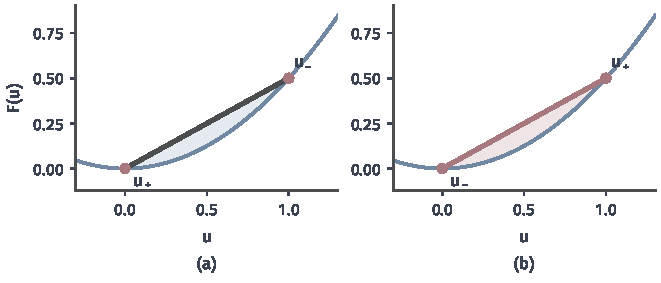
\includegraphics[width=112mm]{figures/06-differential-equations/02-partial-differential-equations/matplotlib/cons-oleinik-chord/figure.pdf}
  \caption{Oleinik条件，$F=u^2/2$（蓝）。两图的弦相同，红点是两个状态。(a)$u_->u_+$，要求图像在弦下方（浅蓝），成立。(b)$u_-<u_+$，要求图像在弦上方，凸函数的图像却在下方（浅红），不成立。}
  \label{fig:cons-oleinik-chord}
\end{BookInlineFigure}

消失黏性的说明到这里还只是形式推导。严格的结论是：$F\in C^1$、$u_0\in L^{\infty}$时，式~\eqref{eq:cons-viscous}的解在$\nu\to0$时在$L^1_{\mathrm{loc}}$中收敛到熵解。证明需要用到解的一致有界性、全变差估计和紧性论证，篇幅较长，读者可查阅Kruzhkov于1970年发表的原始论文或双曲守恒律的专著。这个定理说明熵条件的选择与物理上的小黏性是一致的。
